\documentclass[12pt,a4paper]{report}
\usepackage[utf8]{inputenc}
\usepackage[inner=3.5cm,outer=2.5cm,bottom=3cm,top=2.5cm,pdftex]{geometry}
\usepackage{setspace}
\usepackage{graphicx}
\usepackage{rotating}
\usepackage[page]{appendix}
\usepackage{float}
\usepackage[font=small,labelfont=bf]{caption}
\usepackage{subfigure}
\usepackage{titlesec}
\usepackage[hidelinks]{hyperref}
\usepackage{listings}
\usepackage{textcomp}
\usepackage{fancyhdr}
\usepackage{multirow}
\usepackage{verbatim}	%makes it possible to comment out a section of text by using \begin{comment}...\end{comment}
\usepackage[table,xcdraw]{xcolor}
\usepackage{pifont}
\usepackage{mathptmx}
\usepackage{wrapfig}
\usepackage{ragged2e}
\usepackage[nottoc,notlot,notlof]{tocbibind}
\usepackage[english]{babel}
\usepackage[final]{pdfpages}

\definecolor{rockwoolcolor}{RGB}{105,105,105}

% Style chapter headings for preface and toc.
\setlength{\headheight}{15pt}
\titlespacing*{\chapter}{0pt}{0pt}{4ex}
\titleformat{\chapter}[display]
 {\bfseries\Large}
 {}
 {0pt}
 {\color{rockwoolcolor}\titlerule[2.0pt]\vspace{2ex}\filright\color{black}}
 [\color{rockwoolcolor}\vspace{2ex}{\titlerule[2.0pt]}]


\setstretch{1.25}
\begin{document}
\begin{titlepage}

\newcommand{\HRule}{\color{rockwoolcolor}\rule{\linewidth}{0.75mm}\color{black}} % Defines a new command for the horizontal lines, change thickness here

\center % Center everything on the page
 
%----------------------------------------------------------------------------------------
%	HEADING SECTIONS
%----------------------------------------------------------------------------------------
\ \\[1.5cm]
\textsc{\LARGE BI Handelshøyskolen}\\[1.5cm] % Name of your university/college
\textsc{\Large GRA 41351 Decision Theory and System Dynamics}\\[2.5cm] % Major heading such as course name


%----------------------------------------------------------------------------------------
%	TITLE SECTION
%----------------------------------------------------------------------------------------

\HRule \\[0.4cm]
{ \huge \bfseries Simulation Model for \\[0.5cm] Oslo Municipality}\\[0.4cm] % Title of your document
\HRule \\[2.5cm]
 
%----------------------------------------------------------------------------------------
%	DATE & PLACE SECTION
%----------------------------------------------------------------------------------------

{\large \textbf{Innleveringsdato:}\\  \today}\\[1cm] % Date, change the \today to a set date if you want to be precise
{\large \textbf{Studiested:}\\  BI Nydalen}\\[3cm] % Date, change the \today to a set date if you want to be precise
 
%----------------------------------------------------------------------------------------

\textit{Denne oppgaven er gjennomført som en del av studiet ved Handelshøyskolen BI. Dette innebærer
ikke at Handelshøyskolen BI går god for de metoder som er anvendt, de resultater som er
fremkommet, eller de konklusjoner som er trukket.}
\vfill % Fill the rest of the page with whitespace

\end{titlepage}
{\RaggedRight
\pagestyle{fancy}

% empty default settings for fancy layout
\fancyhf{}

% table mark commands
\newcommand{\cmark}{\textcolor{green!80!black}{\ding{51}}}
\newcommand{\xmark}{\textcolor{red}{\ding{55}}}
\newcommand{\plusmark}{\textcolor{green!80!black}{\textbf{+}}}
\newcommand{\minusmark}{\textcolor{red}{\textbf{-}}}

% chapter, section, header and footer layout
\renewcommand{\sectionmark}[1]{\markright{\thesection ~ \ #1}}
\renewcommand{\chaptermark}[1]{\markboth{ #1}{}}
\renewcommand{\headrulewidth}{0.5pt}
\renewcommand{\footrulewidth}{0.5pt}

%head setting
%\fancyhead[L]{\textcolor{black} {\rightmark}}
\fancyfoot[C]{\textcolor{black} {\thepage}}

% Redefine the plain page style - used when the page is a chapter
\fancypagestyle{plain}{%
  \fancyhf{}%
  \renewcommand{\headrulewidth}{0pt}% Line at the header invisible
  \renewcommand{\footrulewidth}{0.5pt}% Line at the footer visible
  \fancyfoot[C]{\textcolor{black} {\thepage}}
}

% Avoid hyphenating
\tolerance=10
\emergencystretch=\maxdimen
\hyphenpenalty=10000
\hbadness=10000

\pagenumbering{roman}
\chapter*{Summary bla}
The main objective of this paper is analyzing waste sorting behavior and the different factors which influence waste sorting behavior in practice. The reasoning behind this is to help Oslo municipality with reaching a material recycling rate of 50\% by 2030. 

\indent \newline 
The target group consists of 20-39 year old's, not coming from Asia, Africa, Latin-America and Eastern Europe outside of EU. This represents approximately 27\% of all Oslo citizens, and is adjusted for in the simulation model. This means that the model will not be able to reach a realistic material recycling rate of 50\%.

\indent \newline 
A causal loop diagram is presented in order to give an overview of the different variables and their relationships. This includes both positive and negative links on waste sorting behavior. 

\indent \newline 
The simulation model was developed through expanding the existing stocks and flows model with findings from the causal loop diagram. Five initiatives are displayed in the model and consists of increasing advertising effectiveness, increasing the number of waste containers (new quality), implementing smart waste containers (improvements), utilizing economic incentives and increasing frequency of waste collection. The simulations show a "base case" scenario, with a resulting material recycling rate of 31.69\%, while the top three initiatives are increasing the number of waste containers, increasing frequency of waste collection and implementing smart waste containers, with a respectively recycling rate of 36.53\%, 34.4\% and 33.86\%.

\indent \newline 
A sensitivity analysis was performed in order to test the initiatives in different scenarios, which did not the change the recommended suggestions. 

\setcounter{tocdepth}{2}
\tableofcontents
%\addtocontents{toc}{~\hfill\textbf{Page}\par}
\listoffigures
\listoftables

% ----------- CHAPTERS ----------------

% Parts
\cleardoublepage
% Style chapter headings.
\titleformat{\chapter}[display]
 {\bfseries\Large}
 {}
 {0pt}
 {\color{rockwoolcolor}\titlerule[2.0pt]\vspace{2ex}\filright\color{black} \thechapter . }
 [\color{rockwoolcolor}\vspace{2ex}{\titlerule[2.0pt]}]
\pagenumbering{arabic}
\setcounter{page}{1}
\chapter{System Boundaries}
During the last decade, Oslo has been striving to be the next world leading environmentally friendly city when it comes to household recycling. Oslo's main focus is to sustain resources and to achieve a circle-based waste management system. The municipality has for many years been struggling to reach their main goals. In 2006, they set a goal of a 50\% recycling rate by 2014, which evidently turned out unsuccessful \cite{effect}. Oslo municipality was forced to rethink their strategy and extend their goals for further improvements. Oslo municipality now has a goal to reach a 50\% recycling rate for households before 2030, which seems more achievable. This has been deemed an enormous challenge, as there is a stagnating recycling rate in the municipality of Oslo. Today, Oslo has a stable recycling rate of 37\% \cite{oslokommune}.

\indent \newline 
The existing system utilizes three types of garbage bags; a blue bag for plastic, a green bag for food waste and regular plastic bags for rest waste. There is a waste sorting system in-house, which lets the consumer systematically organize their own garbage bags. Regarding curbside collection, there are three different containers; one for plastic and food waste, one for paper/cardboard, and one for rest waste. The frequency of collected waste depends on the area of collection. 

\indent \newline
The main objective of this paper is to analyze the waste sorting behavior of the younger population in Oslo. More specifically, the focus will be on the age group 20-39 year olds and not coming from Asia, Africa, Latin-America and Eastern Europe outside of EU. This particular target group is one of the weakest in terms of household recycling \cite[p. 38]{Mikkelborg}. There are several underlying reasons for this. For instance, this target group often lives in household collectives, which usually consists of a broad mix of people, with different lifestyles and perspectives. If the household lacks cohesiveness, it is very hard to sustain a good recycling behavior. Even though half the household recycles, it would quickly get "un-sorted" by the other half. Secondly, there is a cost associated with waste sorting. Many students and young people have a hard time being financially stable, and any additional household costs would impact their daily life. Finally, the target groups' waste sorting behavior is influenced by time and knowledge. It takes a couple of minutes every day to sort the household waste, which seems small at first, but adds up to a lot. The garbage bags are smaller, which results in taking out the thrash more often. In addition, it is common behavior for this target group to be pessimistic to certain ideas. "It wouldn’t be a noticeable difference if we sort our waste" is a frequent phrase for this target group. There are also several answers to questions they are unaware of, such as the frequency of waste collection and environmental impact of waste sorting. 

\indent \newline
There is, however, a huge potential to improve this target group. With the correct communication, advertisement and incentives through efforts from Oslo municipality, this target group can potentially help Oslo municipality reach their goal within 2030. With a suitable approach, this group can be turned around, which can potentially lead to a higher achieved recycling rate for households in Oslo. 

\indent \newline
The following chapters explains the different variables and factors which influence waste sorting behavior in practice. This includes presenting a causal loop diagram, a stock and flow model, before different initiatives and changes are suggested, in order for Oslo municipality to reach the desired material recycling rate. 



\chapter{Causal Loop Diagram}
In the following part of the paper, the complete causal loop is explained and described in detail. Figure 2.1 displays the whole loop diagram, while the rest of the chapter displays several sub-diagrams. The reasoning behind this is to give a better understanding of the model and to elaborate on the different variables and how they influence waste sorting behavior. 


\begin{figure}[H]
\centering
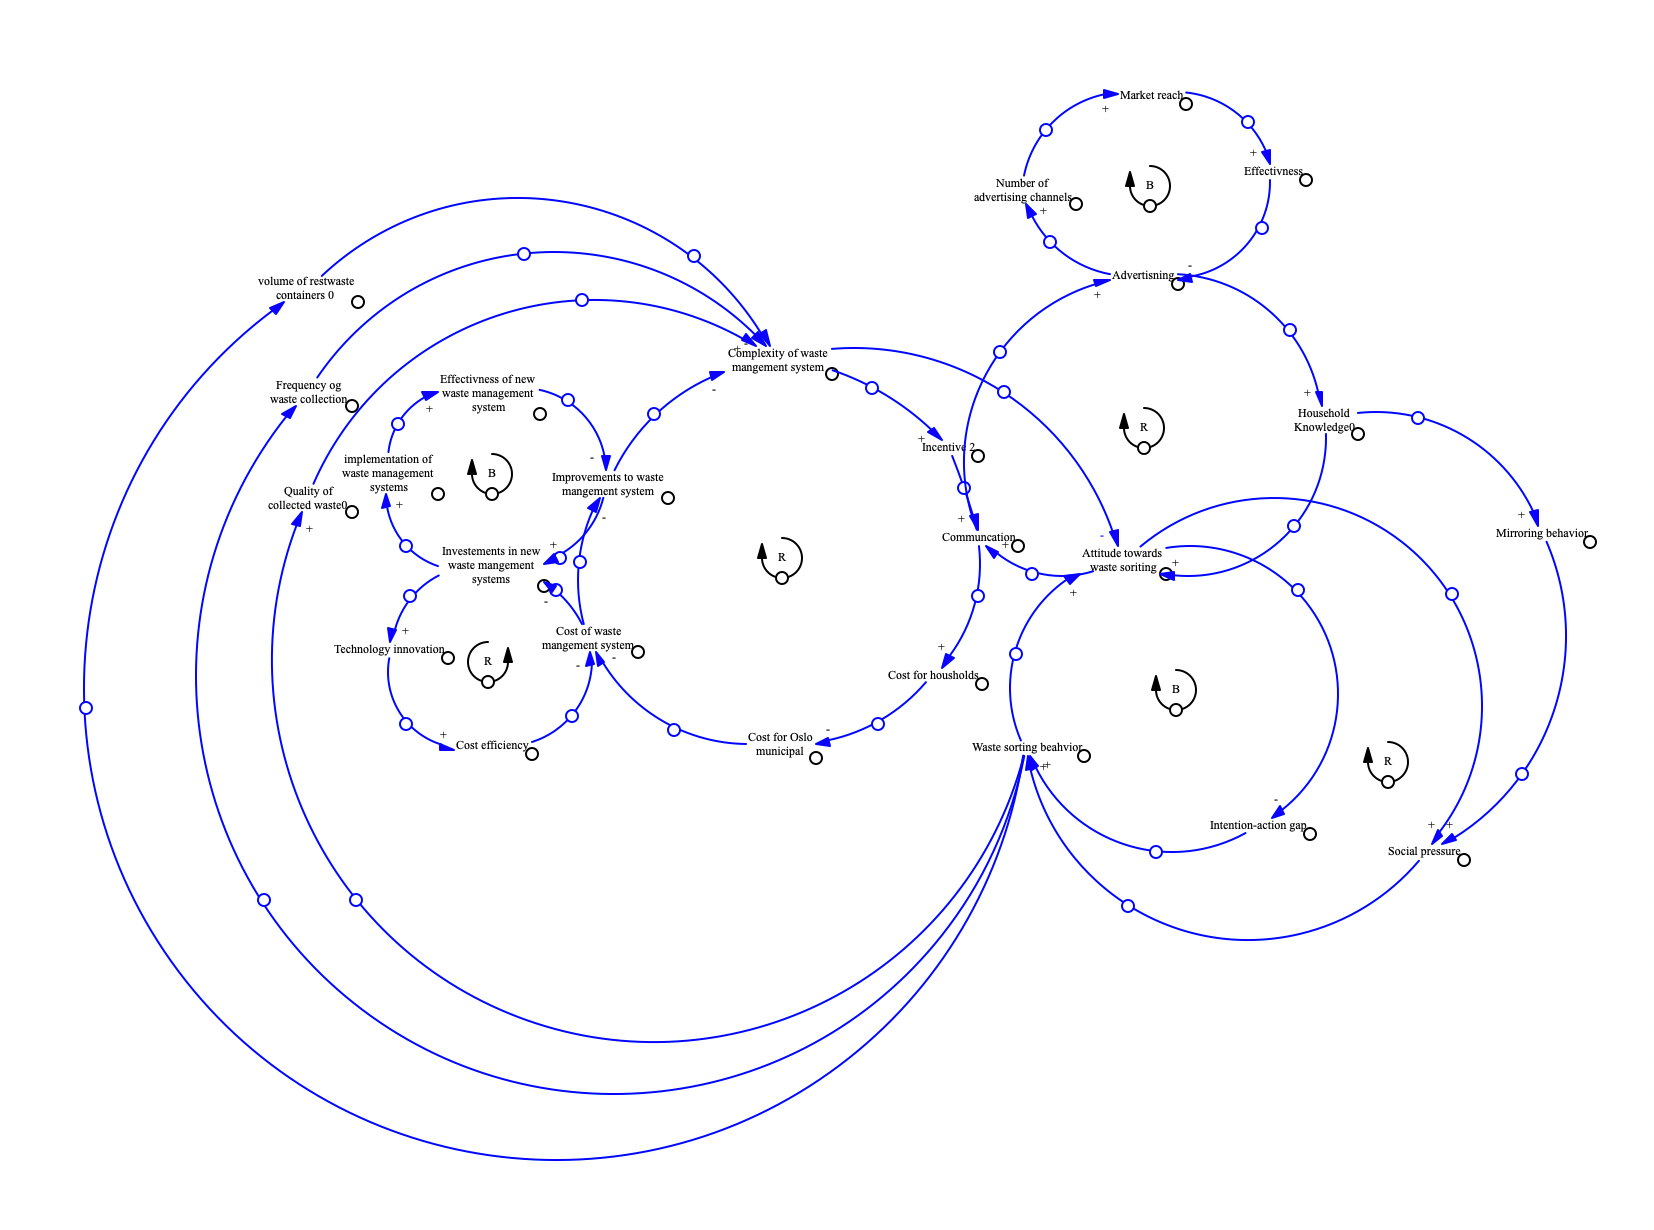
\includegraphics [scale=0.25,angle=90]{figures/fullcld.png}
\caption{Overview of The Causal Loop Diagram}
\label{fig:fullcld}
\end{figure}

\indent \newline
The three central variables in the causal loop diagram is "Quality of collected waste", "Frequency of waste collection" and "volume of rest waste containers". These variables represent initiatives which are among the most important factors in order to improve waste sorting behavior.  

\section{Complexity of Waste Management System}

\begin{figure}[H]
\centering
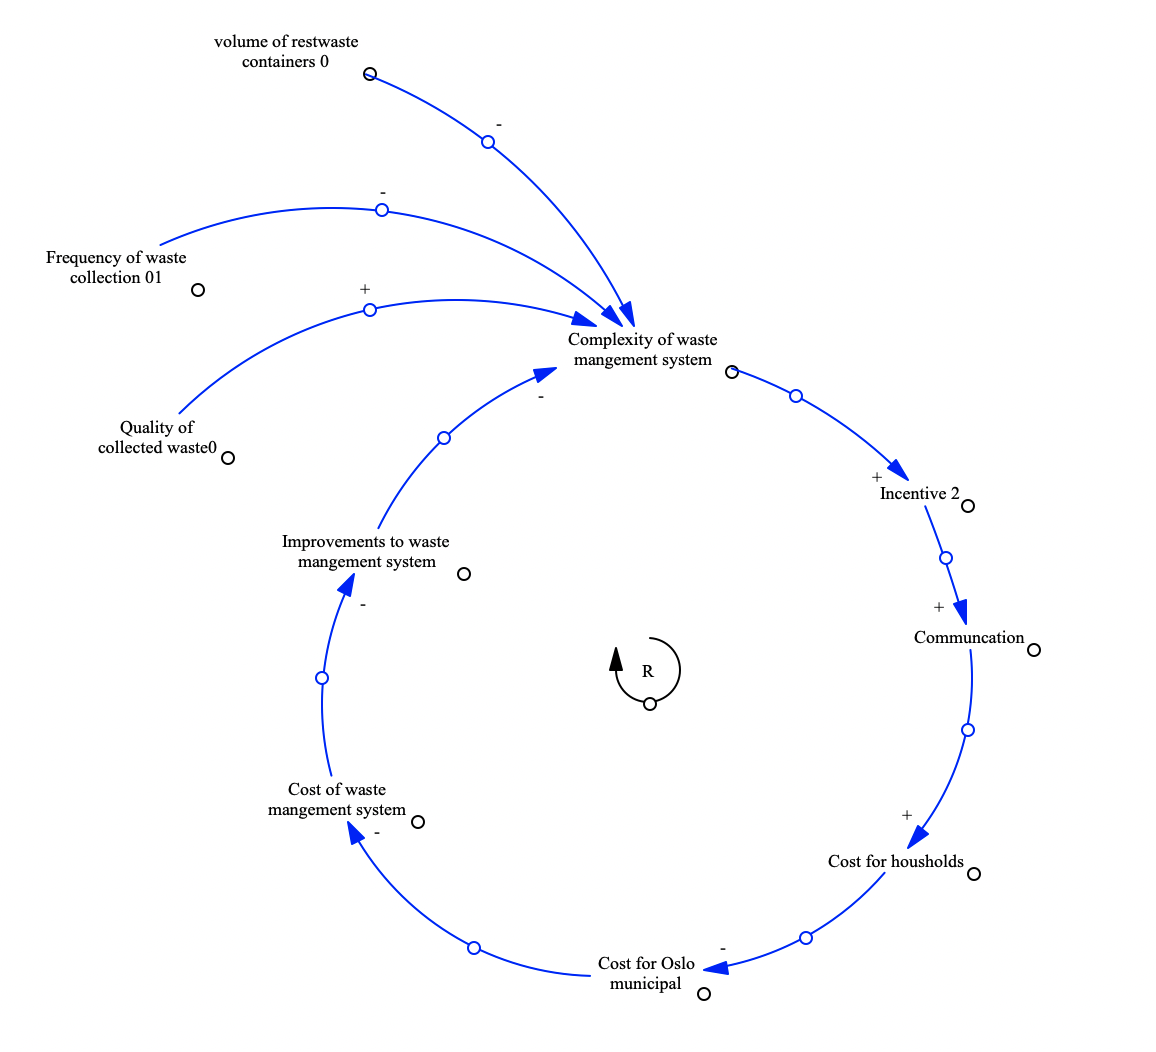
\includegraphics [scale=0.30,angle=360]{figures/complexity.png}
\caption{Complexity of The Waste Management System}
\label{fig:complexity}
\end{figure}

\indent \newline
The complexity of  the waste management system can be interpreted in two different ways.
One is assuming that the citizens have a waste container for each of the materials, which consists of paper, plastic, rest waste and food waste. In this case, Oslo municipality does not have to sort the waste and get rid of the intermediary where the waste is actually sorted. This means that the waste can be sent directly to recycling, which has a significant impact on the complexity of the system. From the citizens point of view, the complexity of the system will rise with the condition of high quality of collected waste. Increasing the frequency of waste collection leads to a less complex waste management system, whereas the citizens avoid bringing the waste back home, presuming the rest waste containers are fully loaded. This also applies to an increase in the volume of rest waste containers. An increase in the complexity of the system means that more incentives are needed on the basis that the citizens have to make more effort to sort properly. Therefore, more incentives mean more communication towards citizens. Possible incentives can presumptive be a fine or financial reward given the quality of the waste sorted.  

\indent \newline
If Oslo municipality increases communication to the citizens, the costs for household will also increase. It has to do with the fact that a percentage of communication costs are charged to households. In this case, the higher the costs for households, the lower the costs for Oslo municipal. The costs for the Oslo municipality are, among other variables, determined through economic incentives, communication and costs related to the waste management system.  

\indent \newline
Assuming an increase in total costs for Oslo municipally, the costs related to the waste management will decrease. This represents a situation where the municipality needs to spend their financial resources on other pressing issues. The next part of the loop shows that an increase in the costs of waste management system will decrease improvements to waste management system. This is a result of a smaller amount of the total budget going towards improvements. Once improvements to waste management systems increase, through technology innovation (explained in Figure 2.6), the complexity of waste management system will decrease. This leads to a reinforcing loop. 

\section{Attitude Towards Waste Sorting}

\begin{figure}[H]
\centering
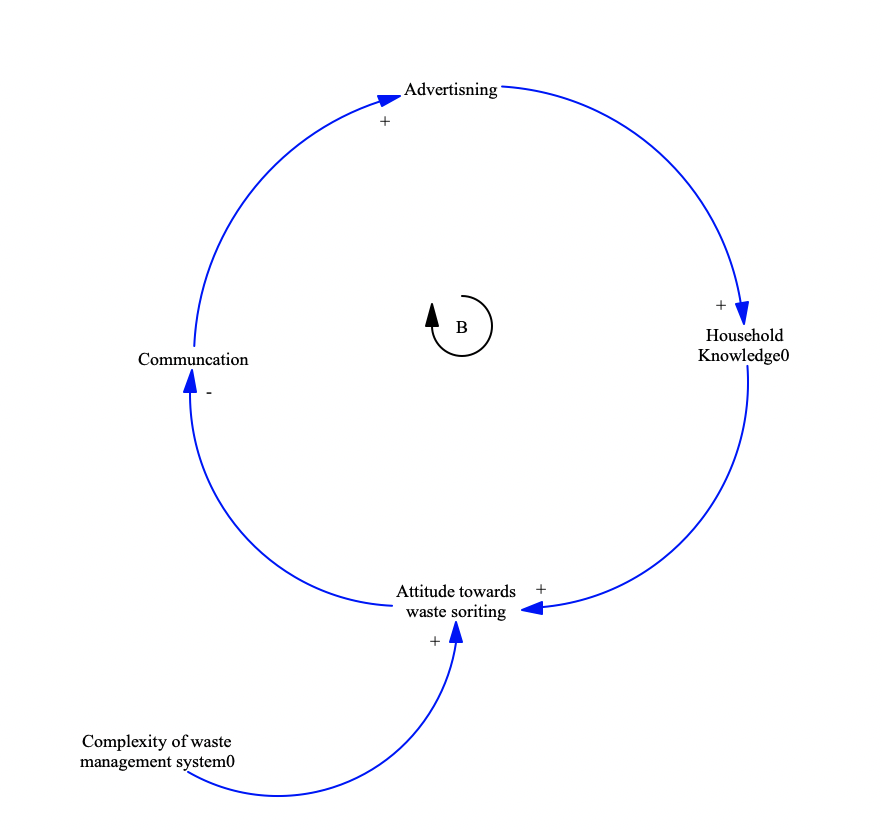
\includegraphics [scale=0.30,angle=360]{figures/attitude.png}
\caption{Attitude Towards Waste Sorting}
\label{fig:attitude}
\end{figure}

\indent \newline
Attitude towards waste sorting is an important variable in the causal loop diagram. The variable both affects and is affected by several variables, and is included in other sub-diagrams as well. Most of the effects related to complexity is explained above, but it also has an effect on the attitude towards waste sorting. If the waste management system increases in complexity, the target group's attitude towards waste sorting will most likely decrease. It is an essential factor for this target group that the waste management system is easy to understand and utilize, and that the workload for the household is minimized. 

\indent \newline
A crucial factor towards increasing the attitude towards waste sorting is household knowledge. When household knowledge is low, it is difficult to have a positive attitude towards waste sorting and vice versa. It is imperative for the target group to acquire knowledge on environmental-impact awareness, as well as the bin system, both curbside and in-house (what goes where). Therefore, it is necessary for the target group to have a reliable source of information in order to acquire a satisfying level of knowledge regarding waste sorting. This will have a positive effect on attitude towards waste sorting.

\indent \newline
There are currently several TV commercials and public posters related to material recycling. However, it is lacking advertising through additional media channels (Figure 2.4). The variables in figure 2.4 are connected through communication, which is a common denominator for the variables mentioned above. This is a simple, but effective balancing loop. If advertising is increased through various media channels, household knowledge will increase, which will lead to an increase in the attitude towards waste sorting. This connects back into communication and will reinforce the relationships even further.

\section{Advertising}

\begin{figure}[H]
\centering
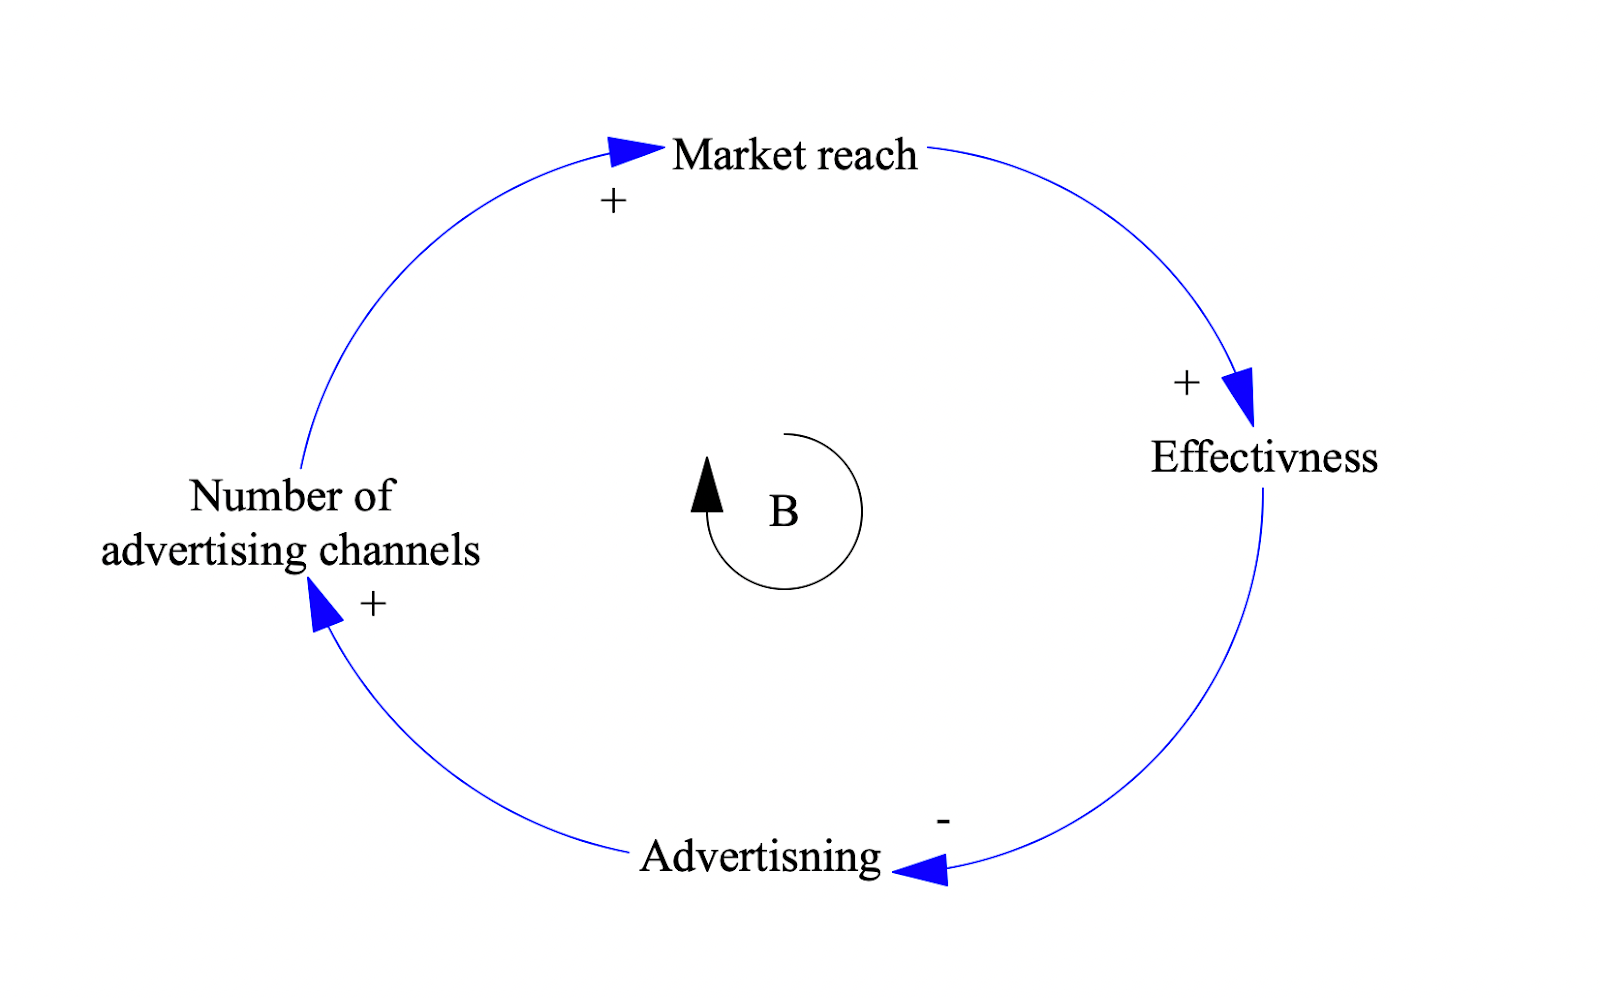
\includegraphics [scale=0.20,angle=360]{figures/advertising.png}
\caption{Advertising}
\label{fig:advertising}
\end{figure}

\indent \newline
In order to achieve the highest market reach within the intended target group, it is necessary to put emphasis on advertising. The target group lacks household knowledge, environmental-impact knowledge and awareness. A potential strategy, in order to reach out to the target group in the most effective way, is communication through various advertising channels. This means focusing on social media campaigns and more traditional advertising channels. Carefully selecting the ideal advertising channels is critical towards maximizing the market reach. Digital platforms such as Facebook, Snapchat, and Instagram is a good place to start. 

\indent \newline
The effect of increasing the number of advertising channels i.e Facebook, Snapchat, Instagram, Twitter, Tumblr, LinkedIn and YouTube, is an increase in market reach within the designated target group. The target group has a vast age interval, and the various social media platforms attract different age groups. Therefore, the more advertising channels, the higher market reach achieved. When the market reach is increased, the resulting outcome will be that the overall effectiveness of our advertising will increase. Once optimal effectiveness is reached, then less advertising is required in order to reach the same results. This part of the diagram results into a balancing loop. 

\section{Social Pressure \& The Intention-Action Gap}

\begin{figure}[H]
\centering
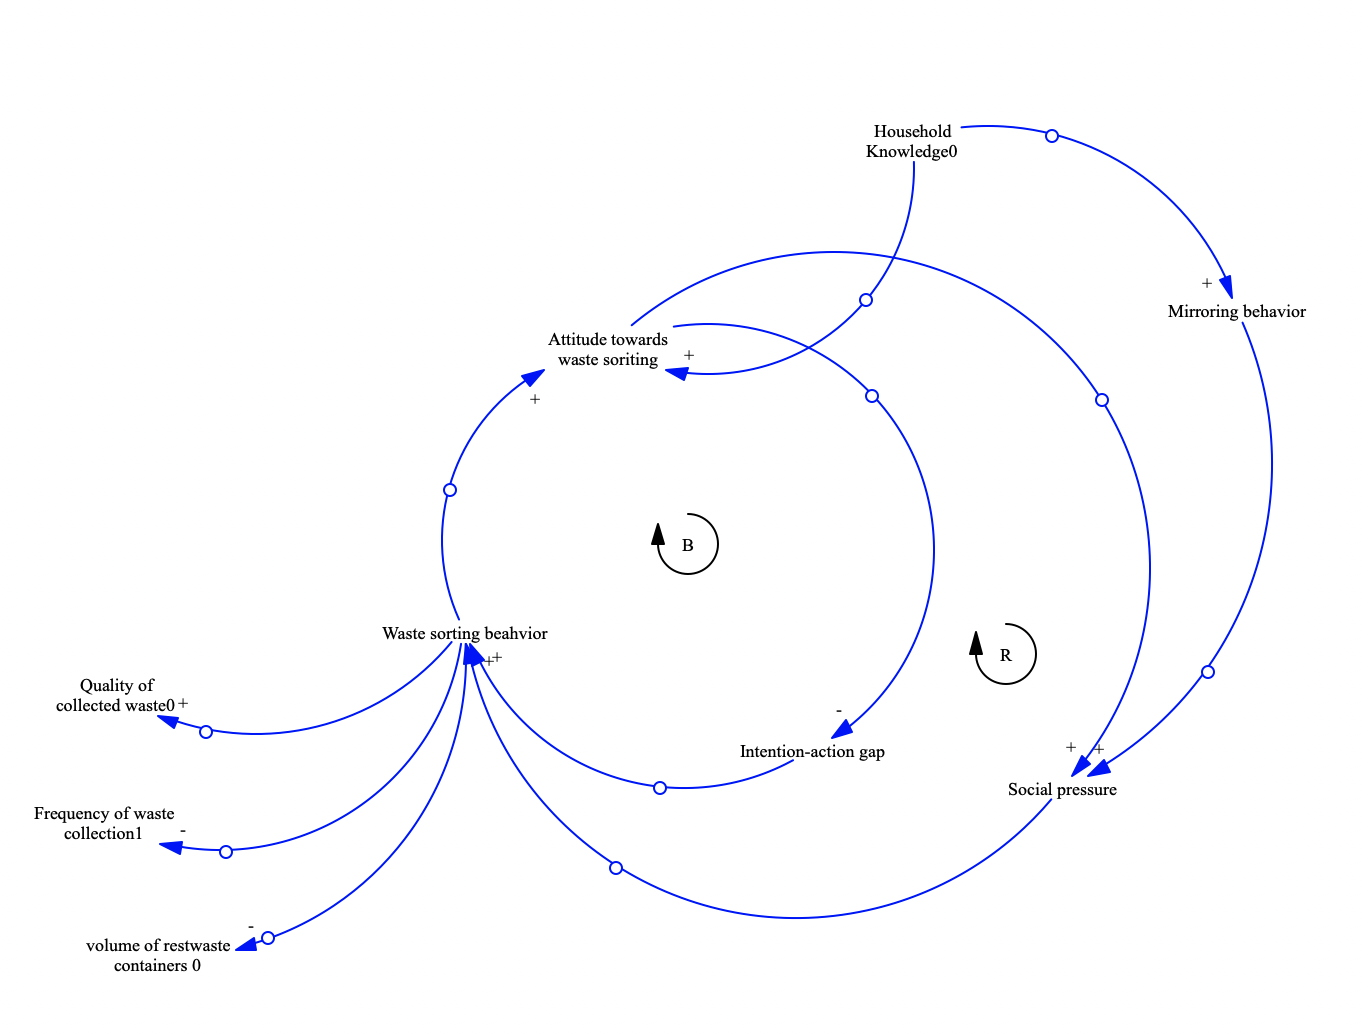
\includegraphics [scale=0.28,angle=360]{figures/socialpressure.png}
\caption{Social Pressure \& The Intention-Action Gap}
\label{fig:Social Pressure}
\end{figure}

\indent \newline
As mentioned formerly, attitude towards waste sorting and household knowledge is two imperative variables in the causal loop diagram, while improving waste sorting behavior is the main objective. However, these variables can lead to both positive and negative effects. 

\indent \newline
An increase in household knowledge will influence a portion of the members in the household to recycle correctly and develop enough awareness of the environmental impact. If one household member starts waste sorting correctly, one can presume that it leads to a mirroring behavior among the other members of the household. According to Jeff Thompson, mirroring behavior is something that occurs subconsciously, especially if we have a positive relationship with the subject \cite{mimicry}. This is often the case in households within this target group, living with either a spouse or friends. In addition, if household knowledge is increased, it will have a positive influence on the attitude towards waste sorting since the subject will be aware of the resulting effects of waste sorting.

\indent \newline
Mirroring behavior has a positive effect on social pressure. It is in our human nature to be sensitive to social pressure, and conform to the values, attitudes or behaviors of others. This can increase individual participation in recycling \cite{shackel}. Individuals will be influenced and encouraged by their fellow peers. This will directly affect their waste sorting behavior. Therefore, if social pressure increases, the waste sorting behavior will also increase.  

\indent \newline
Attitude towards waste sorting will also influence the intention-action gap. The intention-action gap represents the difference between what people say they do, and what they actually do \cite[p. 8]{intention}. Research shows that is common for the target group to have a large intention-action gap when it comes to waste sorting behavior. It amounts to motivation and commitment, which originates from the attitude towards waste sorting. In other words, if there is an increase in attitude towards waste sorting, it will decrease the intention-action gap because people are more committed to the cause. 

\indent \newline
Waste sorting behavior will influence the three variables; "quality of collected waste", "frequency of collected waste" and "volume of rest waste containers". There is a positive relationship between the quality of collected waste and waste sorting behavior. In the case where waste sorting behavior is improved, it will have a direct positive effect on the quality of collected waste. The target group will be more accurate and precise when it comes to waste sorting, which will result in better quality. Regarding the effect of waste sorting behavior on frequency of collected waste, it will have a negative connection. When waste sorting behavior is increased, it will result in less overflow of waste in the containers, which leads to a reduction in frequency of collected waste. It revolves around the household "optimizing" their waste in order to decrease the frequency of collected waste. 

\indent \newline
The relationship between waste sorting behavior and volume of rest waste containers represents the final part of the loop. When waste sorting behavior is increased, it will essentially make more space in the existing containers. The households will optimize their garbage bags, which will result in less excess garbage in various bags.  Therefore, there is a negative relationship between these two variables. 

\section{Improvements to Waste Management System}

\begin{figure}[H]
\centering
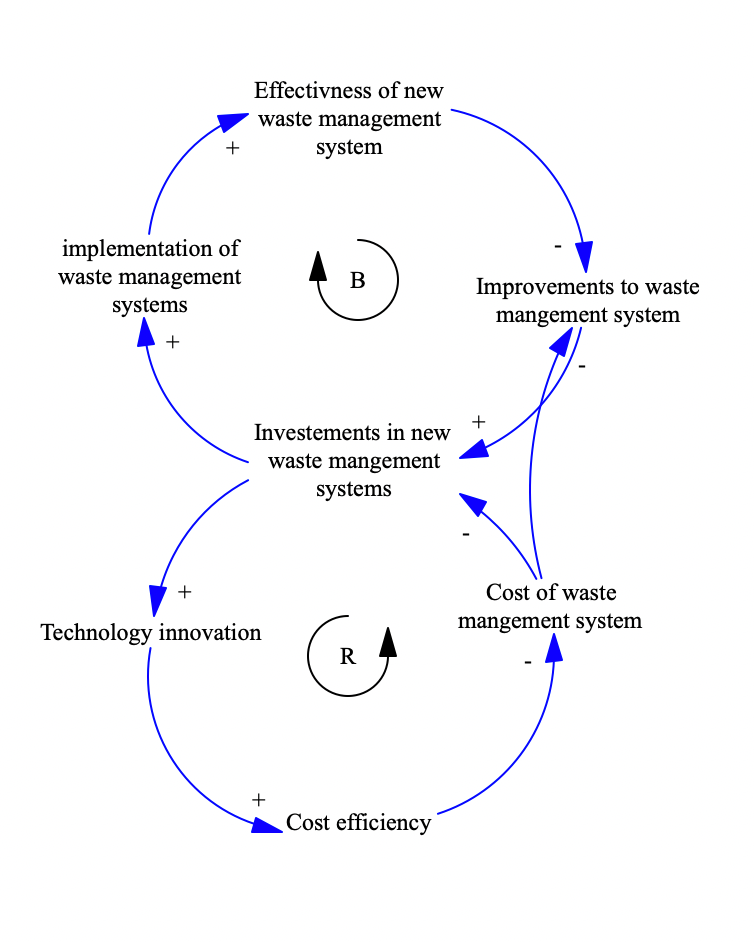
\includegraphics [scale=0.32,angle=360]{figures/improvements.png}
\caption{Improvements to Waste Management System}
\label{fig:improvements}
\end{figure}

\indent \newline
The final part of the causal loop diagram displays the relationships between variables related to how improvements can be made to the current waste management system. In order for this to happen, it is vital to raise enough capital. This can be obtained either from households, through economic incentives or funding from the government. If the effectiveness of the new waste management system increases, there is less need for making improvements to the system. With the condition of an improved sustainable waste management system, an increase in investments is necessary. If investments in the waste management system increases, then  opportunities related to technology innovations will follow. If there is more room to explore new innovations, the cost efficiency will rise, which will result in a decrease in the costs of the waste management system. This feeds back into both the investments in new waste management system and the improvements. The increase of investments leads to implementation of new waste management to establish a more sustainable system for recycling and waste collection. This feeds back into the effectiveness of new management systems, where effectiveness can be measured. The discussed variables and their relationships results into a balancing loop. 

\indent \newline
The causal loop diagram is a visual representation of interdependencies and feedback processes related to the waste management system. The following parts of the paper will convert the diagram into a stock and flow model to measure the resulting effects of proposed solutions, in order for Oslo municipality to reach their recycling goals.


% chapter heading as preface and toc
\titleformat{\chapter}[display]
 {\bfseries\Large}
 {}
 {0pt}
 {\color{rockwoolcolor}\titlerule[2.0pt]\vspace{2ex}\filright\color{black}}
 [\color{rockwoolcolor}\vspace{2ex}{\titlerule[2.0pt]}]
 
\renewcommand\bibname{Referanseliste}
\bibliographystyle{apalike}	% (uses file "plain.bst")
\bibliography{myrefs}		% expects file "mineReferanser.bib"
}

\end{document}
